\documentclass[12pt]{article}
\usepackage{listings}
\usepackage{setspace}
\usepackage{multicol}
\usepackage{enumitem}
\usepackage{amsmath,amsthm,amssymb}
\usepackage[margin=2.5cm]{geometry}
\usepackage{mathtools}
\usepackage{graphicx}
\usepackage{xcolor}
\usepackage{fancyhdr}
\usepackage{hyperref}

% Math stuff
\DeclarePairedDelimiter{\ceil}{\lceil}{\rceil}
\DeclarePairedDelimiter\floor{\lfloor}{\rfloor}

% Image stuff
\graphicspath{ {.} }

% URL Stuff
\hypersetup{
colorlinks=true,
linkcolor=blue,
filecolor=magenta,
urlcolor=cyan,
}

% Header/Foodter setup
\pagestyle{fancy}
\fancyhf{}
\rhead{CSC413 Final Project}
\lhead{Henry Tu and Seel Patel}
\rfoot{Page \thepage}
\lfoot{April 18, 2021}

% Code style setup
\lstdefinestyle{Python}{
language = Python,
frame = lines,
numbers = left,
basicstyle = \scriptsize,
keywordstyle = \color{blue},
stringstyle = \color{green},
commentstyle = \color{red}\ttfamily
}

% To be honest, I have no idea what this is used for
\makeatletter
\renewcommand*\env@matrix[1][*\c@MaxMatrixCols c]{%
\hskip -\arraycolsep
\let\@ifnextchar\new@ifnextchar
\array{#1}}
\makeatother
\onehalfspacing

% Some not sketchy latex
\begin{document}
    \begin{center}
        \textbf{Comparing the interpretability of different GAN architectures}
    \end{center}
    \begin{minipage}{.5\textwidth}
        \centering
        \textbf{Henry Tu}\\
        University of Toronto
    \end{minipage}
    \begin{minipage}{.5\textwidth}
        \centering
        \textbf{Seel Patel}\\
        University of Toronto
    \end{minipage}
    \\

    \begin{multicols*}{2}
        \raggedcolumns

        % Document starts here
        \section{Abstract}
        \label{sec:abstract}
        A Generative Adversarial Network (GAN) uses an adversarial process between two models which are simultaneously trained to estimate a generative model.\cite{gan}
        There are many variants of GAN architectures, such as COCO-GAN\cite{cocogan} and StyleGAN\cite{stylegan}, which both have the ability to generate synthetic images which mimic real images.\\\\
        We are exploring methods of comparing the quantitative performance of these architectures with their interpretability.
        Our quantitative measures include C2ST\cite{evaluateGANs}, image quality measures\cite{evaluateGANs}, etc.\\\\
        In order to analyze these networks qualitatively, we will use methods such as Latent Space Exploration\cite{sampleGAN} and nearest neighbour tests\cite{evaluateGANs} to decipher what the networks have learned.\\\\
        By combining these two forms of analysis, we hope to gain insight into the relationship between performance metrics and the generated output of the models.

        \section{Introduction}
        \label{sec:introduction}
        StyleGAN and COCO-GAN generate images using different techniques to accomplish two different goals: StyleGAN is designed such that high level features of the output image can be finely tuned and adjusted (e.g. lighting, hair colour, etc.)\cite{stylegan}.
        On the other hand, COCO-GAN generates each part of the image separately before stitching it together in order to simulate the human perception of vision\cite{cocogan}.
        As a result, we expected each model to generate images with different qualities that relate to their designed tasks.
        \section{Dataset Generation}
        \label{sec:dataset}
        Both GAN models were trained on the LSUN Bedroom dataset\cite{lsunBedroom} at a resolution of $256 \times 256$.
        Due to time constraints, we used pre-trained models to generate images for our analysis.

        \label{sec:datasetGeneration}
        \subsection{StyleGAN}
        \label{subsec:styleganGeneration}
        NVIDIA Research Projects' Official TensorFlow Implementation of StyleGAN pretrained to the LSUN Bedroom dataset\cite{styleGANCode} was used to generate 5000 images for analysis.
        5000 latent code vectors $\mathbf{z} \in \mathbb{R}^{512}$ drawn from a standard normal distribution which each correspond to an output image.


        \subsection{COCO-GAN}
        \label{subsec:cocoganGeneration}
        \begin{verbatim}placeholder spacer
blah
blah
blah
blah
blah
blah \end{verbatim}
        \section{Quantitative Analysis}
        \label{sec:quantitative}
        \subsection{C2ST}
        \label{subsec:c2st}
        Classifier Two-Sample Tests (C2ST) is used to predict if two samples came from the same distribution\cite{c2st}.
        In the context of evaluating GANs, we will use C2ST to quantitatively measure how well the models mimic real images.
        We trained a deep convolutional neural network to perform binary classification based on the recommended discriminator architecture from \textit{Unsupervised Representation Learning
with Deep Convolutional Generative Adversarial Networks}\cite{dcgan}.
        The goal is to compare the margin by which each GAN model is able to trick the classifier to quantify image generation quality.
        \\\\
        The classifier was implemented in Pytorch with CE loss, the Adam optimizer ($\alpha=0.1$), and the following network architecture:\\
        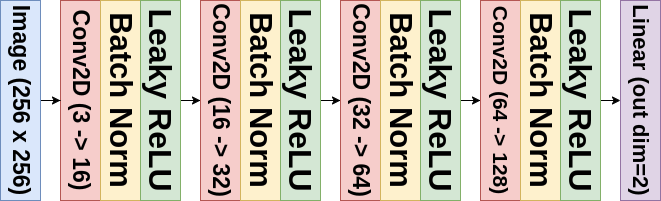
\includegraphics[scale=0.35]{c2st-diagram.png}\\
        \textbf{Kernel Size: 3, Stride: 2, Padding: 1, Leaky ReLU slope: 0.2}.
        Argmax is taken across output of linear units for classification.
        \\\\
        To avoid introducing bias, all three datasets (training, validation, test) were equally balanced with real and generated images (5000 each).
        The generated images were further divided in half between images from StyleGAN and COCO-GAN.
        Out of the combined pool of 10000 images, 5000 were allocated for training, 2500 validation, and 2500 testing.
        \\\\
        The model was trained with a batch size of 200 for 1000 epoches.
        After tuning hyper parameters and performing early stopping with the validation dataset, the following results were attained:
        \\

        \begin{tabular}{ |p{4cm}|p{3cm}|  }
         \hline
         \multicolumn{2}{|c|}{Table 1: Real vs (StyleGAN or COCO-GAN)} \\
         \hline
        Data Set     & Accuracy\\
         \hline
        Training        & 75.9\% of 5000 \\
         \hline
        Validation      & 67.6\% of 2500 \\
         \hline
        Test (Real)     & 58.2\% of 1250 \\
         \hline
        Test (StyleGAN) & 60.5\% of 625  \\
         \hline
        Test (COCO-GAN) & 89.6\% of 625 \\
         \hline
        \end{tabular}
        \\\\
        The model was able to correctly identify the origin of an image the majority of the time.
        This data suggests that StyleGAN is better at tricking the classifier than COCO-GAN.
        \\\\
        To confirm this, we trained additional classifiers using the same architecture, data set distribution, and hyper-parameters but only using images from one of the GAN models.
        (i.e. all 5000 generated images are all from one GAN model)
        The goal is to test how well the classifier performs when isolated to a specific GAN.
        \begin{tabular}{ |p{4cm}|p{3cm}|  }
             \hline
             \multicolumn{2}{|c|}{Table 2: Real vs StyleGAN} \\
             \hline
            Data Set     & Accuracy\\
             \hline
            Training        & 77.6\% of 5000 \\
             \hline
            Validation      & 68.1\% of 2500 \\
             \hline
            Test (Real)     & 74.6\% of 1250 \\
             \hline
            Test (StyleGAN) & 61.4\% of 1250  \\
             \hline
        \end{tabular}
        \begin{tabular}{ |p{4cm}|p{3cm}|  }
             \hline
             \multicolumn{2}{|c|}{Table 3: Real vs COCO-GAN} \\
             \hline
            Data Set     & Accuracy\\
             \hline
            Training        & 87.9\% of 5000 \\
             \hline
            Validation      & 88.2\% of 2500 \\
             \hline
            Test (Real)     & 96.4\% of 1250 \\
             \hline
            Test (COCO-GAN) & 76.1\% of 1250 \\
             \hline
        \end{tabular}
        \\\\
        As seen here, the Real vs COCO-GAN classifier (Table 3) performed significantly better than the Real vs StyleGAN classifier (Table 2).
        This supports the hypothesis that StyleGAN mimics real images better than COCO-GAN.\\\\
        Although these results suggest it is more difficult for a classifier to identify a StyleGAN generated image, it by no means shows that it is impossible to train a more accurate classifier.
        Therefore, we must put the information gathered in the context of the other metrics in order to draw a stronger conclusion.

        \subsection{Image Sharpness}
        \label{subsec:imageSharpness}
        asd

        \subsection{Color Distribution}
        \label{subsec:imageSharpness}
        asd


        \section{Qualitative Analysis}
        \label{sec:qualitative}
        \subsection{Latent Space Exploration}
        \label{subsec:latentSpaceExploration}
        asd
        \subsection{Nearest Neighbours}
        \label{subsec:nearestneighbours}
        asd

        \section{Comparing Results}
        \label{sec:compare}
    \end{multicols*}
    \newpage
    \begin{thebibliography}{9}
        \bibitem{gan}
        Ian J. Goodfellow, Jean Pouget-Abadie, Mehdi Mirza, Bing Xu, David Warde-Farley, Sherjil Ozair, Aaron Courville, and Yoshua Bengio. (2014)
        \href{https://papers.nips.cc/paper/2014/file/5ca3e9b122f61f8f06494c97b1afccf3-Paper.pdf}{\textit{Generative Adversarial Networks} }

        \bibitem{cocogan}
        Chieh Hubert Lin, Chia-Che Chang, Yu-Sheng Chen, Da-Cheng Juan, Wei Wei, Hwann-Tzong Chen. (2019)
        \href{https://arxiv.org/pdf/1904.00284.pdf}{\textit{COCO-GAN: Generation by Parts via Conditional Coordinating} }

        \bibitem{stylegan}
        Tero Karras, Samuli Laine, Timo Aila. (2018)
        \href{https://arxiv.org/pdf/1812.04948.pdf}{\textit{A Style-Based Generator Architecture for Generative Adversarial Networks} }

        \bibitem{evaluateGANs}
        Brownlee, Jason. (2019)
        \href{https://machinelearningmastery.com/how-to-evaluate-generative-adversarial-networks/}{\textit{How to

        \bibitem{sampleGAN}
        Tom White. (2016)
        \href{https://arxiv.org/pdf/1609.04468.pdf}{\textit{Sampling Generative Networks} }

        \bibitem{lsunBedroom}
        Yu, Fisher and Zhang, Yinda and Song, Shuran and Seff, Ari and Xiao, Jianxiong. (2015)
        \href{https://arxiv.org/pdf/1506.03365.pdf}{\textit{LSUN: Construction of a Large-scale Image Dataset using Deep Learning with Humans in the Loop}}

        \bibitem{styleGANCode}
        NVLabs. (2019) \href{https://github.com/NVlabs/stylegan}{\textit{StyleGAN — Official TensorFlow Implementation}}

        \bibitem{c2st}
        David Lopez-Paz, Maxime Oquab. (2016)
        \href{https://research.fb.com/wp-content/uploads/2017/04/neural_tests.pdf?}{\textit{Revisiting Classifier Two-Sample Tests for GAN Evaluation and Causal Discovery}}

        \bibitem{dcgan}
        Alec Radford, Luke Metz, Soumith Chintala. (2015)
        \href{https://arxiv.org/pdf/1511.06434.pdf}{\textit{Unsupervised Representation Learning with Deep Convolutional Generative Adversarial Networks}}

    \end{thebibliography}

\end{document}